\section{Background} \label{sec:background}

% TBD.

\subsection{\paxos}\label{sec:paxos}
% \paxos background. Keys:
% Leader, backup.
% Persistent storage. 
% Network round trips in normal case. Latency.
An SMR system runs the same program and its data on a set of machines 
(replicas), and it uses a distributed consensus protocol (typically, 
\paxos~\cite{paxos:complex,paxos,paxos:simple,paxos:live,paxos:fast,
paxos:practical}) to coordinates inputs across replicas. For efficiency, in 
normal case, \paxos often lets one replica work as the leader which invokes 
consensus requests, and the other replicas work as backups to agree on or 
reject 
these requests. If the leader fails, \paxos elects a new leader from the 
backups.

Two main reliability features must be enforced in a standard \paxos protocol. 
The first one is durability. When a new input comes, the \paxos leader writes 
this input in local stable storage. The leader then starts a new consensus 
round, which invokes a consensus request on ``processing this input" to the 
other backups. A backup also writes the received consensus request in local 
storage if it agrees on this request. Durability ensures that even if the 
leader or backups fail and restart, they can still retrieve the requests from 
local stable storage and re-execute them.

The second feature is safety. As long as a majority of replicas agree on this 
input (\ie, this input is \emph{committed}), \paxos guarantees that all 
replicas consistently agree to process this input. If a replica sees that an 
input consensus has been reached, this consensus must have really been reached 
by at least a majority of replicas. Safety ensures that if a consensus has not 
really been reached, no replica will ``think" that a consensus has been 
reached.

Durability and safety make replicas consistently agree on each input and 
tolerate various faults, including machine failures and network errors. As 
consensus rounds move on, \paxos consistently enforces the same sequence of 
inputs across replicas. It also enforces same execution states across replicas 
without divergence if a program behaves as a deterministic state machine (\ie, 
always produces the same output on the same input).

% Normal case, round trip.
Network latency of consensus messages is one key problem to make general server 
programs adopt SMR. For instance, in an efficient, practical 
\paxos implementation~\cite{paxos:practical}, each input in normal case takes 
one consensus round-trip between every two replicas (one request from the 
leader and one reply from a backup).

\subsection{RDMA} \label{sec:rdma}

RDMA architecture such as Infiniband~\cite{infiniband} or RoCE~\cite{roce} 
recently becomes commonplace in datacenters due to its extreme low latency, 
high throughput, and its decreasing prices. 

RDMA provides three types of communication primitives, from slowest to 
fastest: IPoIB (IP over Infiniband), message verbs, and one-sided read/write 
operations. A one-sided RDMA read/write operation can directly write from one 
replica's memory to a remote replica's memory, completely bypassing OS kernel 
and CPU of the remote replica. For brevity, the rest of this paper denotes a 
one-sided RDMA write operation as a ``WRITE".


% \subsection{State Machine Replication (\smr)} \label{sec:smr}

% State machine replication (\smr) is a powerful fault-tolerance
% concept~\cite{paxos:practical}.  It models a program as a deterministic state 
% machine, where states are important program data and the transitions are 
% deterministic executions of program code under input requests.  \smr runs 
% replicas of this state machine on multiple nodes, tolerating many possible node 
% and network failures.  To keep the replicas consistent, it invokes a
% distributed consensus protocol (typically \paxos~\cite{paxos, paxos:simple, 
% paxos:practical}) to ensure that a quorum (typically majority) of the replicas 
% agree on the input request sequence; under the deterministic execution 
% assumption, this quorum of replicas must reach the same exact state.  \smr is 
% proven safe in theory, and provides high availability in practice.
% 
% To support general server programs transparently, \repbox leverages \repbox's 
% \paxos consensus protocol, which takes the POSIX socket API as
% consensus interface. This \paxos protocol enforces two kinds of 
% orders for socket operations. First, for requests coming from the clients, 
% such as \connect and \send requests, this protocol enforces that all nodes see 
% the same totally ordered sequence of these requests using the \paxos and socket 
% API interposition components.  (this protocol does not need to order the 
% blocking socket operations in the clients because we mainly focus on analyses 
% for server applications.) Second, for server applications' blocking operations, 
% this \paxos protocol schedules them according to the matching operations from 
% the clients (\eg, a \send from a client matches a \recv from the server within 
% the same socket connection). This protocol does not schedule non-blocking 
% operations in servers (\eg, \send to clients) because it focuses on replicating 
% the server's execution states.
% 
% % For practicality, \repbox's \paxos implementation takes a well-known 
% % engineering approach~\cite{paxos:practical}: only the primary invokes consensus 
% % request during normal operations, and an leader election is invoked when 
% % exceptions such as network partitions occur.
% 
% 
% Figure~\ref{fig:repbox} shows an instance of \repbox running on 
% each node, and the \paxos consensus component is the gateway of this instance.  This 
% component accepts socket requests from the clients and invoke a \paxos 
% consensus instance with the other replicas on this operation. Once a consensus 
% is reached, this component forwards the operation to the \dmt component. This 
% component is also the only \repbox component that communicates among different 
% \repbox instances. 
% 
% In this paper, \xxx skips the fault-tolerance nature of \repbox, but leverages it 
% to construct multiple equivalent executions for analysis tools.
% 
% \subsection{Deterministic Multithreading (\dmt)} \label{sec:dmt}
% 
% \dmt~\cite{dpj:oopsla09, 
% dmp:asplos09, kendo:asplos09, coredet:asplos10, dos:osdi10, ddos:asplos13, 
% ics:oopsla13} is an advanced threading technique that enforces the same 
% schedule 
% on the same inputs.  This technique typically maintains a \emph{logical
%   time}\footnote{Though related, the logical time in \dmt is not to be
%   confused with the logical time in distributed
%   systems~\cite{lamportclock}.} that advances deterministically based on
% the code run.  It allows a thread to synchronize only at deterministic
% logical times.  By induction, it makes an entire multithreaded execution
% deterministic.  The overhead of \dmt is typically moderate: one recent
% \dmt system, \parrot~\cite{parrot:sosp13}, incurs an average of 12.7\%
% overhead on a wide range of 108 popular multithreaded programs on 24-core
% machines.
% 
% The \dmt component in Figure~\ref{fig:repbox} runs within the same process as a server replica, and
% enforces the same logical clocks for inter-thread communication
% operations. \repbox leverages the \parrot~\cite{parrot:sosp13} \dmt runtime
% system because it is fast (\ie, 12.7\% overhead for a wide range of 108 popular 
% multithreaded programs) and transparent to the application.
% 
% 
% Specifically, \parrot uses a runtime technique called \ldpreload to dynamically 
% intercept \pthread synchronizations (\eg, \mutexlock) issued by an executable 
% and enforces a well-define, round-robin schedule on these synchronization 
% operations for all threads, practically eliminating nondeterminism in thread
% synchronizations. Although \parrot is not designed to resolve data races
% deterministically, deploying a race detector in one replica can overcome this 
% limitation (\S\ref{sec:discuss}).  \repbox augments the \dmt component to schedule 
% the return points of blocking socket operations in server replicas, too, to 
% ensure that requests are admitted exactly at the same logical time across 
% replicas.



% Our model. Multiple writer multiple reader.
\section{\xxx Overview} \label{sec:overview}

This section first introduces \xxx's architecture design (\S\ref{sec:arch}), 
its workflow on scheduling jobs with replication (\S\ref{sec:workflow}), and 
its trade-off on reliability versus resource consumption (\S\ref{sec:discuss}).

% TBD. 

\subsection{Architecture} \label{sec:arch}

\xxx's deployment model is similar to a typical cluster management system's 
(\eg,~\cite{borg:eurosys15,mesos:nsdi11}). \xxx has a replicas of three to five 
controllers, with each connects with the others using high-speed RDMA network. A 
controller is elected by \paxos as the leading controller, which propose 
consensus requests to execute jobs. The other controllers are standby 
controllers which agree on or reject consensus requests. A number of slave 
machines act as computational resources that hold applications' running jobs. 
Controllers and slaves connect with either RDMA or TCP/IP. Application 
schedulers submit jobs to the leader controller.

\begin{figure}[t]
% \vspace{.20in}
\centering
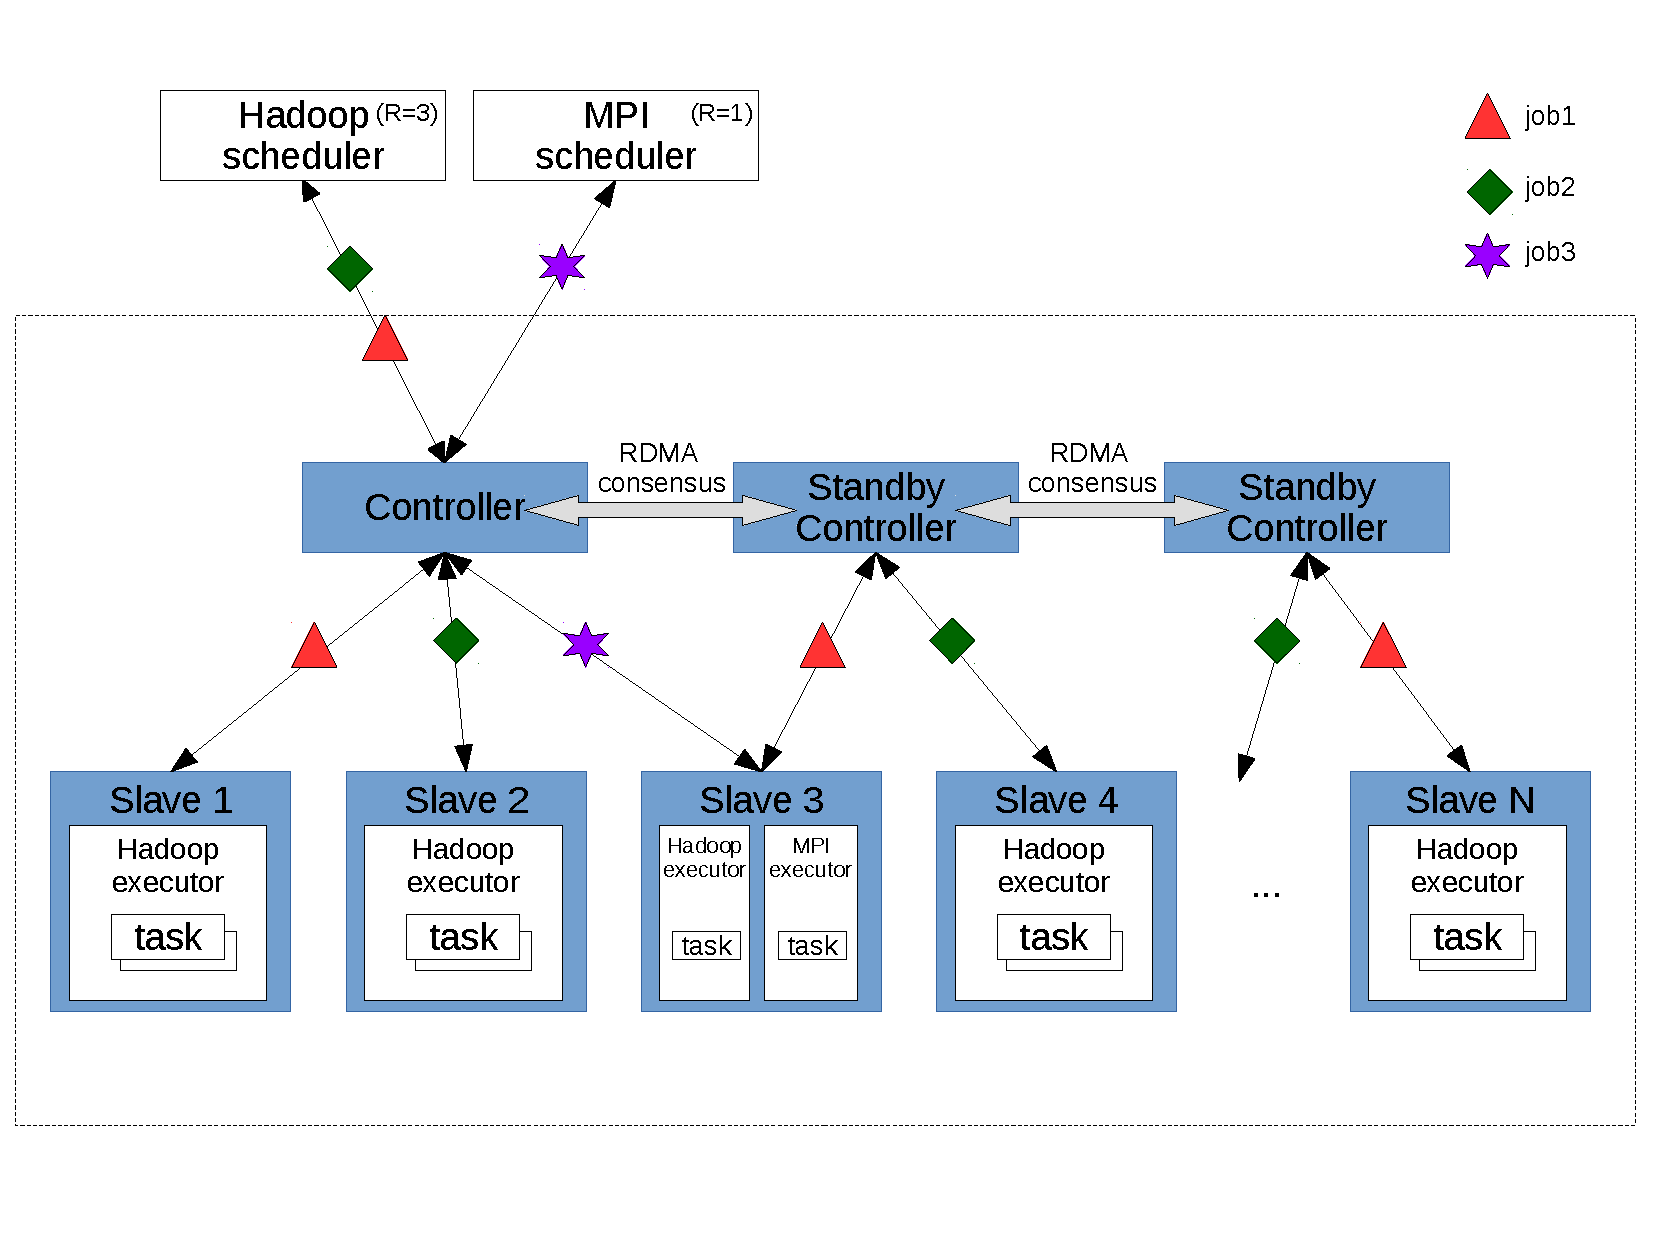
\includegraphics[width=.47\textwidth]{figures/arch}
\vspace{-.2in}
\caption{{\em The \xxx Architecture.} Key components are shaded (and 
in blue).} \label{fig:arch}
\vspace{.05in}
\end{figure}

Figure~\ref{fig:arch} depicts \xxx's architecture, and its key components are 
shaded (and in blue). To illustrate how \xxx works in an application 
perspective, this figure shows two applications, Hadoop and MPI. Each 
application has a \emph{replica strength} (\v{R}) to denote the level of 
fault-tolerance it demands. This value is either 1 or equals the number of 
replicas of controllers in \xxx.

By default, each application has \v{\v{R}=1}, which means that this application 
does not need replication. For such a default setting, \xxx runs the job as is 
without replication, like a typical cluster management system (\eg, Mesos).

In this figure, Hadoop's \v{R} is 3, which means that it wants to replica each 
of its job in three replicas for high-availability. Suppose Hadoop submits two 
jobs to the leader controller, each has different shapes (triangle or 
hexagon). The leader controller thens invokes a consensus on each job across 
controllers. Once a consensus is reached, each controller assigns the same job 
on different slave machines.

The leader controller directly returns its computation result to the Hadoop 
scheduler unless a tail-tolerance mechanism is triggered (\S\ref{sec:workflow}). 
Standby controllers ignore the results unless the same mechanism is triggered.



\subsection{Workflow on Scheduling Jobs} \label{sec:workflow}

Figure~\ref{fig:workflow} shows \xxx's workflow on scheduling jobs with four 
steps. This workflow is similar to that in Mesos except the second and fourth 
steps. These two steps \xxx abstract away the replication logic in its resource 
offers and allocations from the application. An application runs as if \xxx does 
not replicate any of its jobs, and \xxx transparently handles all the 
replication logic.

In the first step, slave machines periodically report their available computing 
resources (\eg, CPU cores and memory) to the leader controller. In the second 
step, instead of reporting available aggregated resources collected from slave 
machines, \xxx divides the amount of resources by each application's \v{R} 
value and then reports to the application. This is to reserve enough resources 
for \xxx to replicate the same job with \v{R} copies.

\begin{figure}[t]
% \vspace{.20in}
\centering
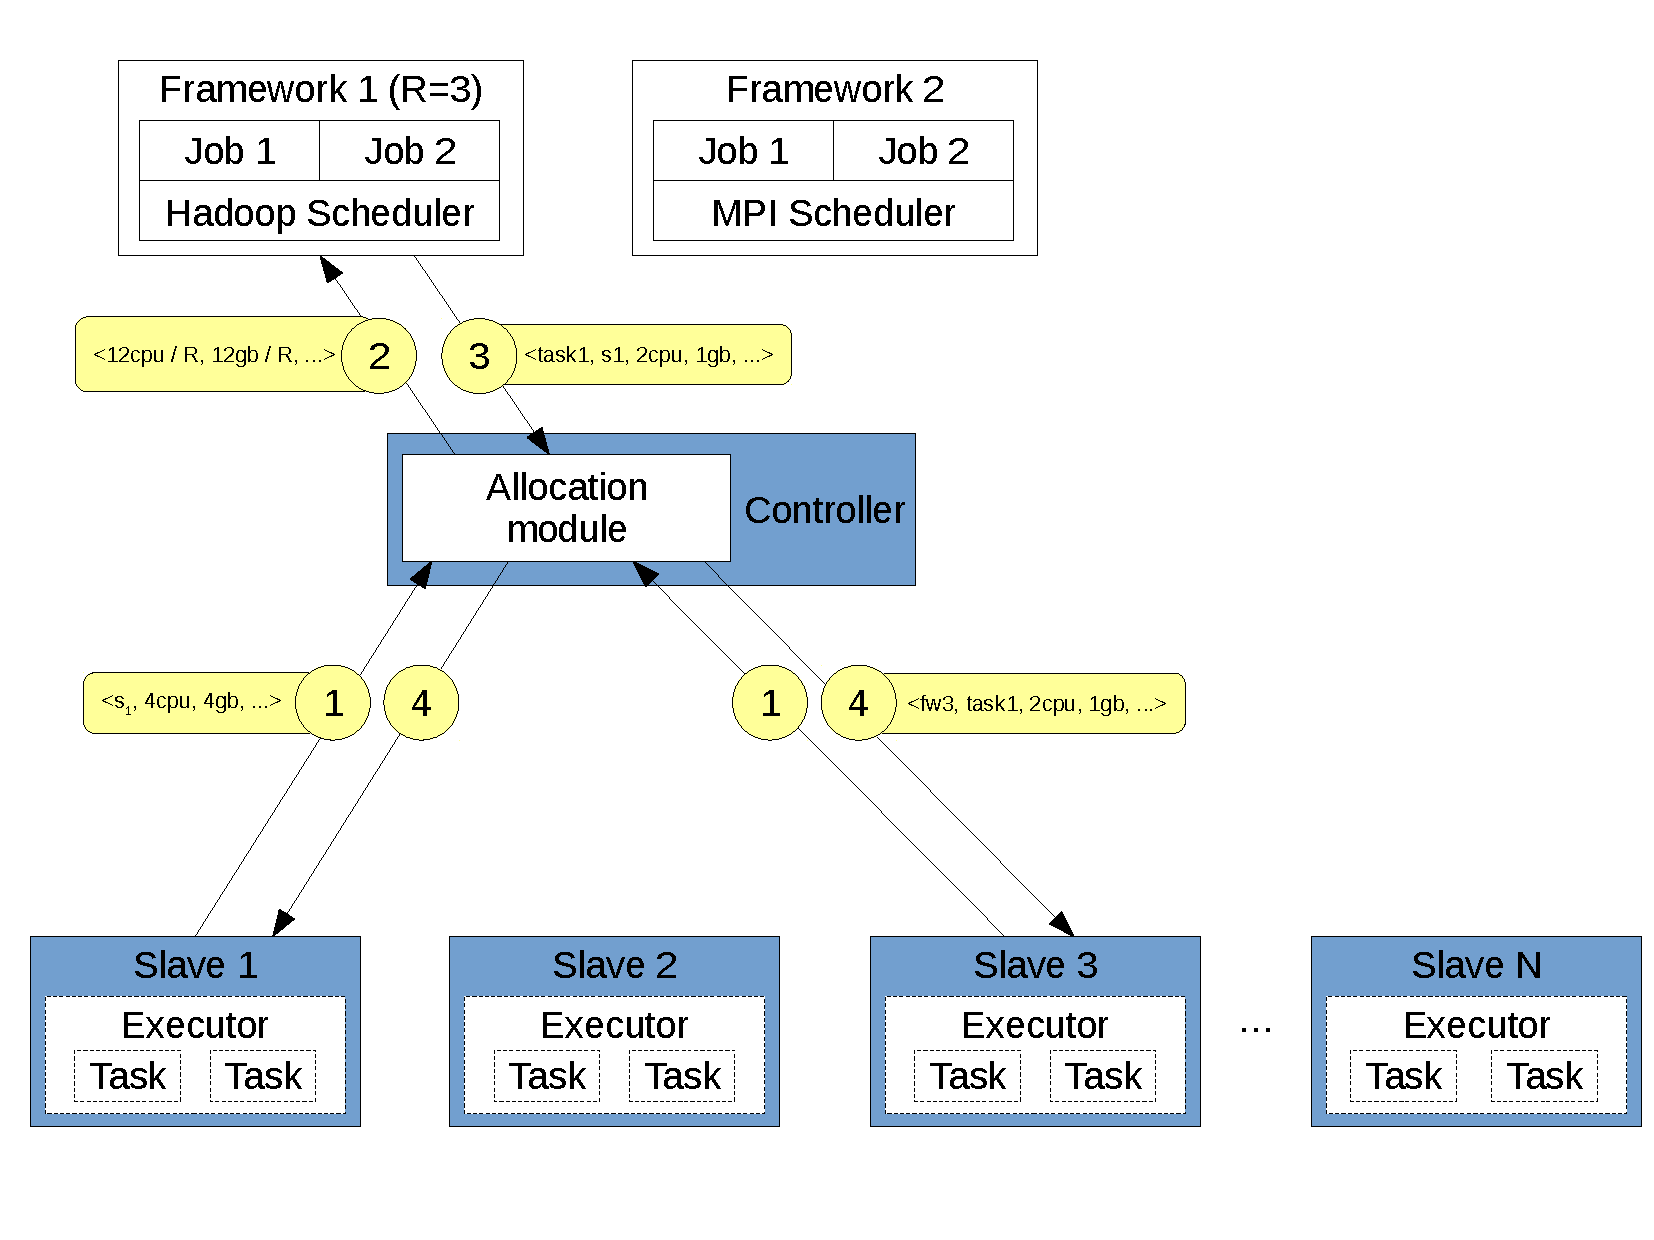
\includegraphics[width=.47\textwidth]{figures/flow}
\vspace{-.2in}
\caption{{\em The \xxx Workflow on Scheduling Jobs.}} \label{fig:workflow}
\vspace{.05in}
\end{figure}

In the third step, an application scheduler submits jobs to the leader 
controller. The leader controller then invokes a consensus on this job by 
carrying the resource offer made to the application.

Once a majority of controllers agrees on executing this job, each controller 
does the fourth step. It schedules this job on an available slave machine 
according to the resource offer. To avoid controllers putting the same job on 
the same slave machine, each controller maintains a disjoint bit-mask of slave 
machines; it only schedules this job on machines belongs to its bit-mask if 
this machine has available resource to hold this job.

% More discussions, frangmentation, 4+1+1, not available to hole 3*2. 
% But critical applications, resource is often not a bottleneck compared to 
% response time and availability.

\subsection{Discussion} \label{sec:discuss}

The main goal of \xxx is to provide high-availability to critical applications 
running in clusters. On one hand, clusters are included more and more computing 
resources (\eg, machines), where failures of these resources and applications 
are already commonplace~\cite{facebook:outage}. On the other hand, 
high requirements on response times and availability become more and more 
important to critical applications.

For instance, Both NYSE and Nasdaq have experienced outage of their whole 
site~\cite{nyse:halt} or specific IPO events~\cite{facebook:ipo:delay} due to 
minor machine errors.  Even social-networking applications like Facebook has 
strong fault-tolerance requirements, because minor machine failures have turned 
down the whole Facebook site for several times in the last few 
years~\cite{facebook:outage}, costing huge 
money lost. 

Therefore, \xxx's design favors more on availability and performance 
(low consensus latency). It's design tends to use \v{R} times of resources 
compared to traditional applications. We argue that this extra resource 
utilizations are acceptable for critical applications, because if they have high 
demand on availability and response times, they can often tolerate costs on 
computing resources (\eg, trading and medical platforms).


\section{Tail-tolerance Design} \label{sec:tail}

\xxx's tail tolerance design is based on its \paxos consensus protocol. This 
design consists of three steps. First, for each job request, both the leader 
controller and standby controllers schedule the same job and receive output of 
this job. When each standby controller receives a job output, it 
uses RDMA WRITEs to write back their job outputs to the leader master's local 
memory.

Second, the leader master also waits for its own job output and frequently 
polls from the other replicas' outputs for this job. Third, if the leader finds 
that standby masters have already written back an output for a job, it sends 
back the output to the application scheduler and ignores its own job output. 
This guarantees that application schedulers receive job outputs without being 
affected by stragglers in minor replicated jobs.

Although \xxx is not the first work that presents a replication approach to 
address the straggler problem (\eg, Dolly~\cite{dolly:nsdi13}), \xxx's 
tail-tolerance design has two practical benefits. First, \xxx's design is 
simple and general to applications, because it is built on top of its \paxos 
replication architecture without extra replication logic. Second, the standby 
masters' output write-back are fast through RDMA writes. 
